% Generated by experiments/make_figures.py.
\definecolor{cA}{HTML}{2a78d6}\definecolor{cB}{HTML}{eb6834}\definecolor{cC}{HTML}{1baf7a}%
\definecolor{cD}{HTML}{4a3aa7}\definecolor{cGray}{HTML}{8a8984}%
\definecolor{lvA}{HTML}{c6dbf5}\definecolor{lvB}{HTML}{93bbec}\definecolor{lvC}{HTML}{5e98e0}%
\definecolor{lvD}{HTML}{2a78d6}\definecolor{lvE}{HTML}{174a8c}\definecolor{lvF}{HTML}{1baf7a}%
\begin{figure*}
  \centering
  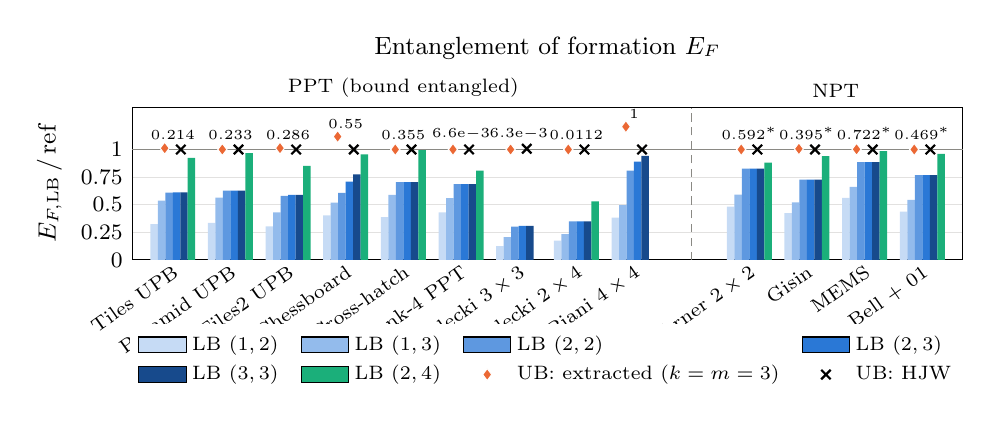
\begin{tikzpicture}
    \begin{axis}[width=\textwidth, height=0.29\textwidth, ymin=0, ymax=1.38, xmin=0.30000000000000004, xmax=14.7,
      ylabel={$E_{F,\mathrm{LB}}\,/\,$ref}, ytick={0,0.25,0.5,0.75,1}, xtick={1,2,3,4,5,6,7,8,9,11,12,13,14},
      xticklabels={{Tiles UPB},{Pyramid UPB},{GenTiles2 UPB},{Chessboard},{Cross-hatch},{Rank-4 PPT},{Horodecki $3\times3$},{Horodecki $2\times4$},{Piani $4\times4$},{Werner $2\times2$},{Gisin},{MEMS},{Bell + $\ket{01}$}}, xticklabel style={rotate=35, anchor=north east, font=\scriptsize, inner sep=1pt},
      tick label style={font=\footnotesize}, label style={font=\small}, title={Entanglement of formation $E_F$}, title style={font=\small,
      yshift=8pt}, clip=false, legend style={font=\scriptsize, at={(0.5,-0.42)}, anchor=north, legend columns=4, draw=none, /tikz/every even column/.append style={column sep=6pt}}, legend cell align=left,
      ytick style={draw=none}, xtick style={draw=none}, ymajorgrids, grid style={cGray!25}]
            \addplot[ybar, bar width=0.13, bar shift=0pt, draw=none, fill=lvA, area legend] coordinates {(0.675,0.324904) (1.675,0.334656) (2.675,0.303153) (3.675,0.404005) (4.675,0.388144) (5.675,0.431027) (6.675,0.123997) (7.675,0.174286) (8.675,0.381966) (10.675,0.482983) (11.675,0.423665) (12.675,0.562028) (13.675,0.437146)};\addlegendentry{LB $(1,2)$}
      \addplot[ybar, bar width=0.13, bar shift=0pt, draw=none, fill=lvB, area legend] coordinates {(0.805,0.537373) (1.805,0.565058) (2.805,0.430906) (3.805,0.517956) (4.805,0.589725) (5.805,0.559301) (6.805,0.205242) (7.805,0.232661) (8.805,0.496878) (10.805,0.592167) (11.805,0.521884) (12.805,0.661474) (13.805,0.544231)};\addlegendentry{LB $(1,3)$}
      \addplot[ybar, bar width=0.13, bar shift=0pt, draw=none, fill=lvC, area legend] coordinates {(0.935,0.610045) (1.935,0.627155) (2.935,0.580622) (3.935,0.606008) (4.935,0.705062) (5.935,0.686084) (6.935,0.302016) (7.935,0.349271) (8.935,0.809017) (10.935,0.827902) (11.935,0.728126) (12.935,0.886515) (13.935,0.767598)};\addlegendentry{LB $(2,2)$}
      \addplot[ybar, bar width=0.13, bar shift=0pt, draw=none, fill=lvD, area legend] coordinates {(1.065,0.61083) (2.065,0.627155) (3.065,0.588493) (4.065,0.709303) (5.065,0.705062) (6.065,0.687289) (7.065,0.308418) (8.065,0.349271) (9.065,0.890301) (11.065,0.827902) (12.065,0.728126) (13.065,0.886515) (14.065,0.767598)};\addlegendentry{LB $(2,3)$}
      \addplot[ybar, bar width=0.13, bar shift=0pt, draw=none, fill=lvE, area legend] coordinates {(1.195,0.610888) (2.195,0.627155) (3.195,0.589237) (4.195,0.774563) (5.195,0.705062) (6.195,0.68729) (7.195,0.308447) (8.195,0.349271) (9.195,0.943262) (11.195,0.827902) (12.195,0.728126) (13.195,0.886515) (14.195,0.767598)};\addlegendentry{LB $(3,3)$}
      \addplot[ybar, bar width=0.13, bar shift=0pt, draw=none, fill=lvF, area legend] coordinates {(1.325,0.923362) (2.325,0.966867) (3.325,0.85094) (4.325,0.95686) (5.325,0.993487) (6.325,0.809194) (8.325,0.530762) (11.325,0.881576) (12.325,0.940658) (13.325,0.98508) (14.325,0.959485)};\addlegendentry{LB $(2,4)$}
            \addplot[only marks, mark=diamond*, mark size=2.2pt, cB, mark options={draw=white, line width=0.4pt}] coordinates {(0.86,1.01207) (1.86,1) (2.86,1.01258) (3.86,1.11694) (4.86,1) (5.86,1) (6.86,1) (7.86,1.00004) (8.86,1.20691) (10.86,1) (11.86,1.0061) (12.86,1.00195) (13.86,1.00003)};\addlegendentry{UB: extracted ($k=m=3$)}
      \addplot[only marks, mark=x, mark size=2.4pt, black, thick] coordinates {(1.14,1) (2.14,1) (3.14,1) (4.14,1) (5.14,1) (6.14,1.00003) (7.14,1.00708) (8.14,1) (9.14,1) (11.14,1) (12.14,1) (13.14,1) (14.14,1)};\addlegendentry{UB: HJW}
      \draw[cGray] (axis cs:0.30000000000000004,1) -- (axis cs:14.7,1);
      \node[anchor=south, font=\tiny, inner sep=1pt] at (axis cs:1,1.06) {$0.214$};
      \node[anchor=south, font=\tiny, inner sep=1pt] at (axis cs:2,1.06) {$0.233$};
      \node[anchor=south, font=\tiny, inner sep=1pt] at (axis cs:3,1.06) {$0.286$};
      \node[anchor=south, font=\tiny, inner sep=1pt] at (axis cs:4,1.157) {$0.55$};
      \node[anchor=south, font=\tiny, inner sep=1pt] at (axis cs:5,1.06) {$0.355$};
      \node[anchor=south, font=\tiny, inner sep=1pt] at (axis cs:6,1.06) {$6.6\mathrm{e}{\scriptscriptstyle-3}$};
      \node[anchor=south, font=\tiny, inner sep=1pt] at (axis cs:7,1.06) {$6.3\mathrm{e}{\scriptscriptstyle-3}$};
      \node[anchor=south, font=\tiny, inner sep=1pt] at (axis cs:8,1.06) {$0.0112$};
      \node[anchor=south, font=\tiny, inner sep=1pt] at (axis cs:9,1.247) {$1$};
      \node[anchor=south, font=\tiny, inner sep=1pt] at (axis cs:11,1.06) {$0.592^*$};
      \node[anchor=south, font=\tiny, inner sep=1pt] at (axis cs:12,1.06) {$0.395^*$};
      \node[anchor=south, font=\tiny, inner sep=1pt] at (axis cs:13,1.06) {$0.722^*$};
      \node[anchor=south, font=\tiny, inner sep=1pt] at (axis cs:14,1.06) {$0.469^*$};
      
      \draw[cGray, densely dashed] (axis cs:10,0) -- (axis cs:10,1.38);\node[font=\scriptsize, anchor=south] at (axis cs:5,1.38) {PPT (bound entangled)};\node[font=\scriptsize, anchor=south] at (axis cs:12.5,1.38) {NPT};
    \end{axis}
  \end{tikzpicture}
  \caption{Lower bounds on the entanglement of formation for different PPT and NPT states, from the SDP with embedded LP (Sec.~\ref{sec:LP}). Bars: lower bounds from the simplified hierarchy at the levels $(k,m)$ shown in the legend. Markers: upper bounds from the decomposition extracted from the SDP solution at $k=m=3$ (orange) and from HJW gradient descent over decompositions (black). All values are divided by the reference printed above each state: the exact convex roof for two qubits (marked $^*$), and the lowest of the two upper bounds otherwise. The gap closes as the level of the hierarchy increases.
  The level $(2,4)$ is missing for the Horodecki $3\times3$ and the Piani $4\times4$ states, since their rank is too high and the SDP exceeded the memory of our machine.}
  \label{fig:EoF}
\end{figure*}